\documentclass[9pt,a4paper,twocolumn,twoside]{rho-class/rho}
\usepackage[english]{babel}
% \usepackage{placeins}

%----------------------------------------------------------
% TITLE INFO
%----------------------------------------------------------
\title{Determinant Quantum Monte Carlo Simulation of the 2D Hubbard Model}
\author{Dhruv Dua}
\author{Dumbre Anuj}
\author{Ishit Ranjan}
\affil{IISER Bhopal}
\date{April 2026}
\doctype{Project Report}

%----------------------------------------------------------
% PACKAGES
%----------------------------------------------------------
\usepackage{amsmath}
\usepackage{amssymb}
\usepackage{physics}
\usepackage{graphicx}
\usepackage{bm}
\usepackage{hyperref}

%----------------------------------------------------------
% ABSTRACT
%----------------------------------------------------------
\begin{abstract}
This report presents a Determinant Quantum Monte Carlo (DQMC) study of the two-dimensional Hubbard model on a $4\times4$ periodic lattice at half filling. The Hubbard model is a minimal microscopic description of interacting electrons on a lattice and provides a central framework for understanding magnetism, Mottness, and correlation-driven phase transitions. In the present work, DQMC is used to compute thermodynamic observables as a function of interaction strength $U/t$, including double occupancy, local magnetic moments, and interaction energy. The method relies on a first-order Trotter decomposition of the imaginary-time evolution operator, a discrete Hubbard-Stratonovich transformation, and stabilized propagation of fermionic Green's functions via QR decomposition with column pivoting. The numerical results show the expected suppression of double occupancy and the expected growth of local moments with increasing repulsion. The report also discusses Trotter discretization errors, finite-size limitations, and the numerical stabilization required for reliable long imaginary-time simulations.
\end{abstract}

\keywords{DQMC, Hubbard Model, Quantum Monte Carlo, Strong Correlations, Hubbard-Stratonovich Transformation}

\begin{document}
\maketitle

\tableofcontents
\listoffigures
\vspace{15pt}
\begin{tcolorbox}[colback=rhocolor!13, arc=3pt, boxrule=0pt, left=6pt, right=6pt, top=2pt, bottom=2pt, before skip=0pt, after skip=2pt]
\centering
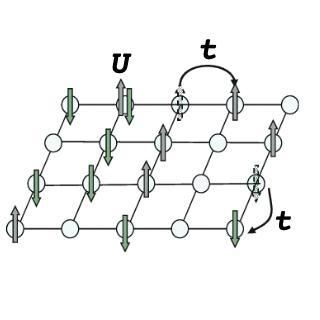
\includegraphics[width=0.92\columnwidth]{uploads/t(1).png}
\captionof{figure}[Schematic of the two-dimensional Hubbard model]{Schematic of the two-dimensional Hubbard model used in this report. Electrons hop between nearest-neighbor lattice sites with amplitude $t$, while the on-site repulsion $U$ penalizes double occupancy. Image adapted from Susumu Yamada, Toshiyuki Imamura, and Masahiko Machida, licensed under CC BY-SA 4.0 via Wikimedia Commons; colors were modified for this report.}
\label{fig:firstpage-hubbard}

\end{tcolorbox}
\vspace{5pt}
\noindent\textbf{Acknowledgment.} The authors gratefully acknowledge Dr.~Sunil Pratap Singh and the Department of Physics, IISER Bhopal, for providing the opportunity and academic environment in which this project was carried out.

\clearpage

%----------------------------------------------------------
\section{Introduction}
%----------------------------------------------------------

The Hubbard model is one of the most important models in condensed matter physics because it captures the competition between itinerancy and local repulsion in the simplest possible lattice setting. Despite its apparent simplicity, it exhibits a rich variety of physical phenomena including antiferromagnetism, Mott insulating behavior, local-moment formation, and the emergence of strong correlation effects in low-dimensional systems. At half filling on a bipartite lattice, the model is especially important because particle-hole symmetry simplifies the physics and makes the finite-temperature formulation especially clean.

The standard two-dimensional square-lattice Hubbard model is widely used as a benchmark system for numerical many-body methods. It serves as a prototype for strongly correlated electron systems and is also a model of conceptual relevance in the study of cuprates and other unconventional superconductors. At finite temperature, Determinant Quantum Monte Carlo (DQMC) provides a numerically exact method, up to systematic Trotter error and finite-size effects, for sampling the fermionic partition function \cite{blankenbecler1981,hirsch1983,white1989}.

In this project, we simulate the Hubbard model on a $4\times4$ lattice with periodic boundary conditions. The goal is to study how observables evolve as the interaction strength increases and to connect the numerical trends with the underlying many-body physics.

%----------------------------------------------------------
\section{Model and Physical Picture}
%----------------------------------------------------------

The repulsive Hubbard Hamiltonian is

\begin{equation}
H = -t \sum_{\langle i,j\rangle,\sigma}
\left(c^\dagger_{i\sigma}c_{j\sigma} + c^\dagger_{j\sigma}c_{i\sigma}\right)
+ U \sum_i n_{i\uparrow}n_{i\downarrow}-\mu\sum_i(n_{i\uparrow}+n_{i\downarrow})
\end{equation}

where $t$ is the nearest-neighbor hopping amplitude, $U$ is the on-site Coulomb repulsion, $c^\dagger_{i\sigma}$ creates a fermion of spin $\sigma$ at site $i$, and $n_{i\sigma}=c^\dagger_{i\sigma}c_{i\sigma}$.\, $\mu \rightarrow$Chemical potential term that controls the filling of the $e^-s$.

% \begin{figure}[t]
%     \centering
%     \includegraphics[width=0.6\linewidth]{uploads/t (1).png}
%     \caption{Schematic representation of the two-dimensional Hubbard model. 
%     Electrons hop between nearest-neighbor sites with amplitude $t$, while 
%     on-site interaction $U$ penalizes double occupancy.}
%     \label{fig:hubbard_model}
% \end{figure}

The first term favors delocalization and metallic behavior, while the second term penalizes double occupation and drives the system toward localization. These two competing effects define the central physics of the model. In the weak-coupling regime $U/t \ll 1$, kinetic energy dominates. In the strong-coupling regime $U/t \gg 1$, the electrons become more localized and an effective spin model emerges in the low-energy limit.

At half filling, the model is particularly important because the average density is one electron per site. On a bipartite lattice with periodic boundary conditions, the repulsive Hubbard model at half filling has an exact particle-hole symmetry. This symmetry suppresses charge imbalance and simplifies the structure of the finite-temperature problem. In our implementation, half filling is enforced by fixing the chemical potential at $\mu = 0$, which is consistent with particle-hole symmetry on the square lattice.

%----------------------------------------------------------
\subsection{Strong-Coupling Limit}
%----------------------------------------------------------

In the limit $U/t \gg 1$, virtual hopping processes generate an effective antiferromagnetic exchange interaction between neighboring spins. To leading order in $t/U$, the low-energy theory becomes the Heisenberg model with exchange coupling

\begin{equation}
J = \frac{4t^2}{U}.
\end{equation}

This result provides a key physical interpretation of the strong-coupling regime: charge fluctuations are suppressed, but spin fluctuations survive and order becomes primarily magnetic rather than metallic. The appearance of local moments is therefore a direct signature of interaction-driven localization. In this regime, the double occupancy is reduced and the local spin degree of freedom becomes more pronounced.

The interaction-driven crossover from itinerant electrons to local moments is one of the main qualitative outcomes that DQMC should reproduce. For a half-filled square lattice, increasing $U$ suppresses charge fluctuations and makes local-moment formation more pronounced.

%----------------------------------------------------------
\section{DQMC Method}
%----------------------------------------------------------

The finite-temperature partition function is

\begin{equation}
Z = \mathrm{Tr}\left(e^{-\beta H}\right),
\end{equation}

with inverse temperature $\beta = 1/(k_B T)$. DQMC evaluates this quantity by writing the imaginary-time evolution operator as a product of short-time factors. Splitting the Hamiltonian into kinetic and interaction parts, $H=K+V$, the first-order Trotter decomposition gives

\begin{equation}
e^{-\beta H}
=
\left(e^{-\Delta\tau K}e^{-\Delta\tau V}\right)^L
+ O(\Delta\tau),
\end{equation}

where $\beta=L\Delta\tau$. The inverse temperature $\beta$ is therefore not an independent input but is determined by the number of time slices $L$ and the imaginary-time step $\Delta\tau$. The error from this approximation is systematic and vanishes as $\Delta\tau \to 0$ \cite{blankenbecler1981}.

The decomposition is essential because the hopping and interaction operators do not commute. Once the Hamiltonian is discretized in imaginary time, the interacting fermion problem can be transformed into a sum over auxiliary-field configurations. A useful broader review of the numerical linear-algebra issues that arise in Hubbard-model quantum Monte Carlo is given in \cite{bai2009}.

%----------------------------------------------------------
\subsection{Hubbard-Stratonovich Transformation}
%----------------------------------------------------------

The quartic interaction term prevents direct analytic integration over fermionic degrees of freedom. DQMC resolves this by introducing an auxiliary Hubbard-Stratonovich (HS) field, which decouples the interaction into a problem of noninteracting fermions moving in a fluctuating field. For the discrete Ising decoupling,

\begin{equation}
e^{-\Delta\tau U(n_\uparrow n_\downarrow - \frac{n_\uparrow+n_\downarrow}{2})}
=
\frac{1}{2} \sum_{s=\pm1}
e^{\lambda s(n_\uparrow-n_\downarrow)},
\end{equation}

where $\lambda$ is defined through

\begin{equation}
\cosh(\lambda)=e^{U\Delta\tau/2}.
\end{equation}

This form is especially convenient at half filling because it preserves spin symmetry and, on bipartite lattices, avoids the sign problem for the repulsive Hubbard model. After introducing the HS field, the fermions can be integrated out exactly, leaving a determinant weight for each auxiliary-field configuration \cite{hirsch1983,blankenbecler1981}. The implementation tracks the sign of each determinant explicitly throughout the simulation, accumulating observables weighted by the sign product of both spin sectors.

The HS field is initialized at the start of the simulation as a random configuration of $\pm 1$ values over all sites and time slices. The results are independent of this initial condition after a sufficient number of equilibration sweeps, which are discarded before measurements begin.

%----------------------------------------------------------
\subsection{Monte Carlo Formulation}
%----------------------------------------------------------

For a given auxiliary-field configuration $s$, the partition function becomes

\begin{equation}
Z = \sum_{\{s\}} \det M_\uparrow(s)\det M_\downarrow(s),
\end{equation}

where

\begin{equation}
M_\sigma(s) = I + B^\sigma_L B^\sigma_{L-1}\cdots B^\sigma_1.
\end{equation}

The matrices $B^\sigma_\ell$ represent propagation through one imaginary-time slice. Their dependence on the HS field means that the auxiliary spin configuration controls the effective fermion dynamics. The Monte Carlo algorithm proposes local updates to the HS field and accepts or rejects them based on the resulting change in determinant weight.

The equal-time Green's function is given by

\begin{equation}
G^\sigma = \left(I + B^\sigma_L\cdots B^\sigma_1\right)^{-1}.
\end{equation}

This matrix contains the one-body information needed to compute observables such as density, double occupancy, and local moments. Efficient rank-1 Sherman-Morrison updates greatly reduce the cost of successive field updates. After all sites at a given time slice have been visited, the Green's function is propagated forward to the next time slice before the sweep continues. In addition to equal-time quantities, the implementation also stores the imaginary-time displaced Green's functions $G^\sigma(\tau, 0)$ for all time slices, which provide access to dynamic correlators and spectral information in future extensions of the work.

%----------------------------------------------------------
\subsection{Algorithmic Workflow}
%----------------------------------------------------------

A typical DQMC simulation proceeds as follows:

\begin{enumerate}
\item Initialize an auxiliary-field configuration with random $\pm 1$ values.
\item Compute Green's functions from the full product of time-slice propagators.
\item For each time slice, propose a local flip of the auxiliary field at each site and accept or reject the update using the Metropolis criterion. The acceptance probability is $P = \min(1,\, |d_\uparrow\, d_\downarrow|)$, where $d_\sigma$ is the determinant ratio for spin sector $\sigma$. The sign of the weight is tracked separately.
\item After sweeping all sites at a time slice, propagate the Green's function forward to the next time slice.
\item Periodically recompute the Green's function from scratch via stabilized QR decomposition to prevent numerical drift.
\item After equilibration, measure observables and average over Monte Carlo samples.
\end{enumerate}

Because DQMC samples the partition function stochastically, results become more accurate as the number of sweeps increases, although statistical errors remain finite.

%----------------------------------------------------------
\subsection{Numerical Stabilization}
%----------------------------------------------------------

The product of many imaginary-time evolution matrices becomes numerically ill-conditioned at large $\beta$. This is a well-known issue in DQMC because repeated multiplication amplifies roundoff errors and can destroy linear independence in the propagated basis. To control this problem, stabilized propagation is essential.

In our implementation, stabilization follows the algorithm of Bai et al.\ \cite{bai2009}, in which QR decompositions with column pivoting are interleaved into the chain of $B$-matrix products. The matrix chain is divided into blocks of a fixed length, and a QR factorization is applied at the boundary of each block. This bounds the growth of the condition number and prevents overflow and underflow in the propagated Green's function. Two Green's function routines are used: a fast direct inversion for intermediate updates and a fully stabilized decomposition-based recomputation for periodic correction. Without this stabilization, the computed Green's functions would become unreliable after sufficiently many time slices.

For long simulations, stabilization is not an optional refinement but a necessary part of the algorithm. The need for this step becomes more severe as the interaction strength or inverse temperature increases. Performance-critical routines, including the inner Monte Carlo loop and the measurement accumulation, are compiled using Numba's just-in-time compiler, which provides near-native execution speeds without leaving the Python ecosystem.

%----------------------------------------------------------
\section{Measured Observables}
%----------------------------------------------------------

Several observables are particularly useful for diagnosing the physics of the Hubbard model.

\paragraph{Double Occupancy.}

The double occupancy is defined as

\begin{equation}
D = \langle n_\uparrow n_\downarrow \rangle.
\end{equation}

It measures the probability that two electrons of opposite spin occupy the same site. Since the on-site repulsion penalizes this configuration, $D$ decreases as $U/t$ increases. In the weak-coupling limit, $D$ is relatively large; in the strong-coupling limit, it becomes suppressed. In the implementation, $D$ is accumulated per site and averaged over all sites to give a translationally averaged quantity.

\paragraph{Local Magnetic Moment.}

The local moment is

\begin{equation}
m_z^2 = \langle (n_\uparrow - n_\downarrow)^2 \rangle
= \langle n_\uparrow + n_\downarrow - 2n_\uparrow n_\downarrow \rangle.
\end{equation}

This quantity increases as double occupancy decreases, reflecting the formation of localized spins. It is one of the clearest indicators of correlation-driven magnetism in the Hubbard model. Like the double occupancy, it is measured per site and averaged over the lattice.

\paragraph{Interaction Energy.}

The interaction energy is

\begin{equation}
E_{\mathrm{int}} = U\sum_i \langle n_{i\uparrow}n_{i\downarrow}\rangle.
\end{equation}

For a translationally invariant system, this is proportional to $UD$. It provides direct information about the cost of charge fluctuations and is therefore closely tied to the suppression of double occupancy. The total energy is not directly measured in the present implementation; kinetic-energy measurements are left as a future improvement.

%----------------------------------------------------------
\section{Simulation Setup}
%----------------------------------------------------------
The calculations were performed using the following parameters:

\begin{itemize}
\item Lattice sizes: $2\times2$ (validation) and $4\times4$ (results)
\item Boundary condition: periodic
\item Filling: half filling ($\mu = 0$)
\item Hopping amplitude: $t=1$
\item Interaction strengths: $U/t = 0,1,2,3,4,5,6,7,8$
\item Imaginary-time step: $\Delta\tau=0.1$
\item Number of time slices: $L=40$ ($\beta = L\Delta\tau = 4$)
\item Equilibration sweeps: 1000
\item Measurement sweeps: 2000
\end{itemize}

The $2\times2$ system was used to validate the implementation against exact diagonalization results, while the $4\times4$ lattice was used to study the dependence of observables on interaction strength. The framework additionally supports parallel execution over parameter sweeps and persistent storage of results in HDF5 format, though all results presented here were obtained with serial execution and in-memory output.

%----------------------------------------------------------
\section{Validation via Exact Diagonalization}
%----------------------------------------------------------
To verify the correctness of the DQMC implementation, simulations were performed on a $2\times2$ lattice and compared with exact diagonalization results obtained using the QuSpin library at the same inverse temperature $\beta = 4$.

The double occupancy computed using DQMC was found to agree closely with the exact results over the full range of interaction strengths. This agreement confirms that the implementation correctly reproduces the thermodynamic properties of the Hubbard model at finite temperature for small system sizes.

This validation step provides confidence that the algorithm, including the Trotter decomposition, the random initialization of the HS field, and the Monte Carlo sampling, is functioning as intended.

\begin{figure}[t]
\centering
\includegraphics[width=\columnwidth]{uploads/exact vs monte carlo.pdf}
\caption{Comparison of exact diagonalization (ED) and determinant quantum Monte Carlo (DQMC) results for the double occupancy on the $2\times2$ Hubbard lattice at half filling and inverse temperature $\beta = 4$. The close agreement validates the DQMC implementation.}
\label{fig:ed-vs-dqmc}
\end{figure}

% %----------------------------------------------------------
% \section{Results and Physical Interpretation}
% %----------------------------------------------------------

% The results are consistent with the expected physics of the repulsive Hubbard model at half filling. As $U/t$ increases, double occupancy decreases because doubly occupied sites become energetically costly. At the same time, local moments grow because electrons preferentially avoid each other and occupy different sites.


% \begin{figure*}[t]
% \centering

% 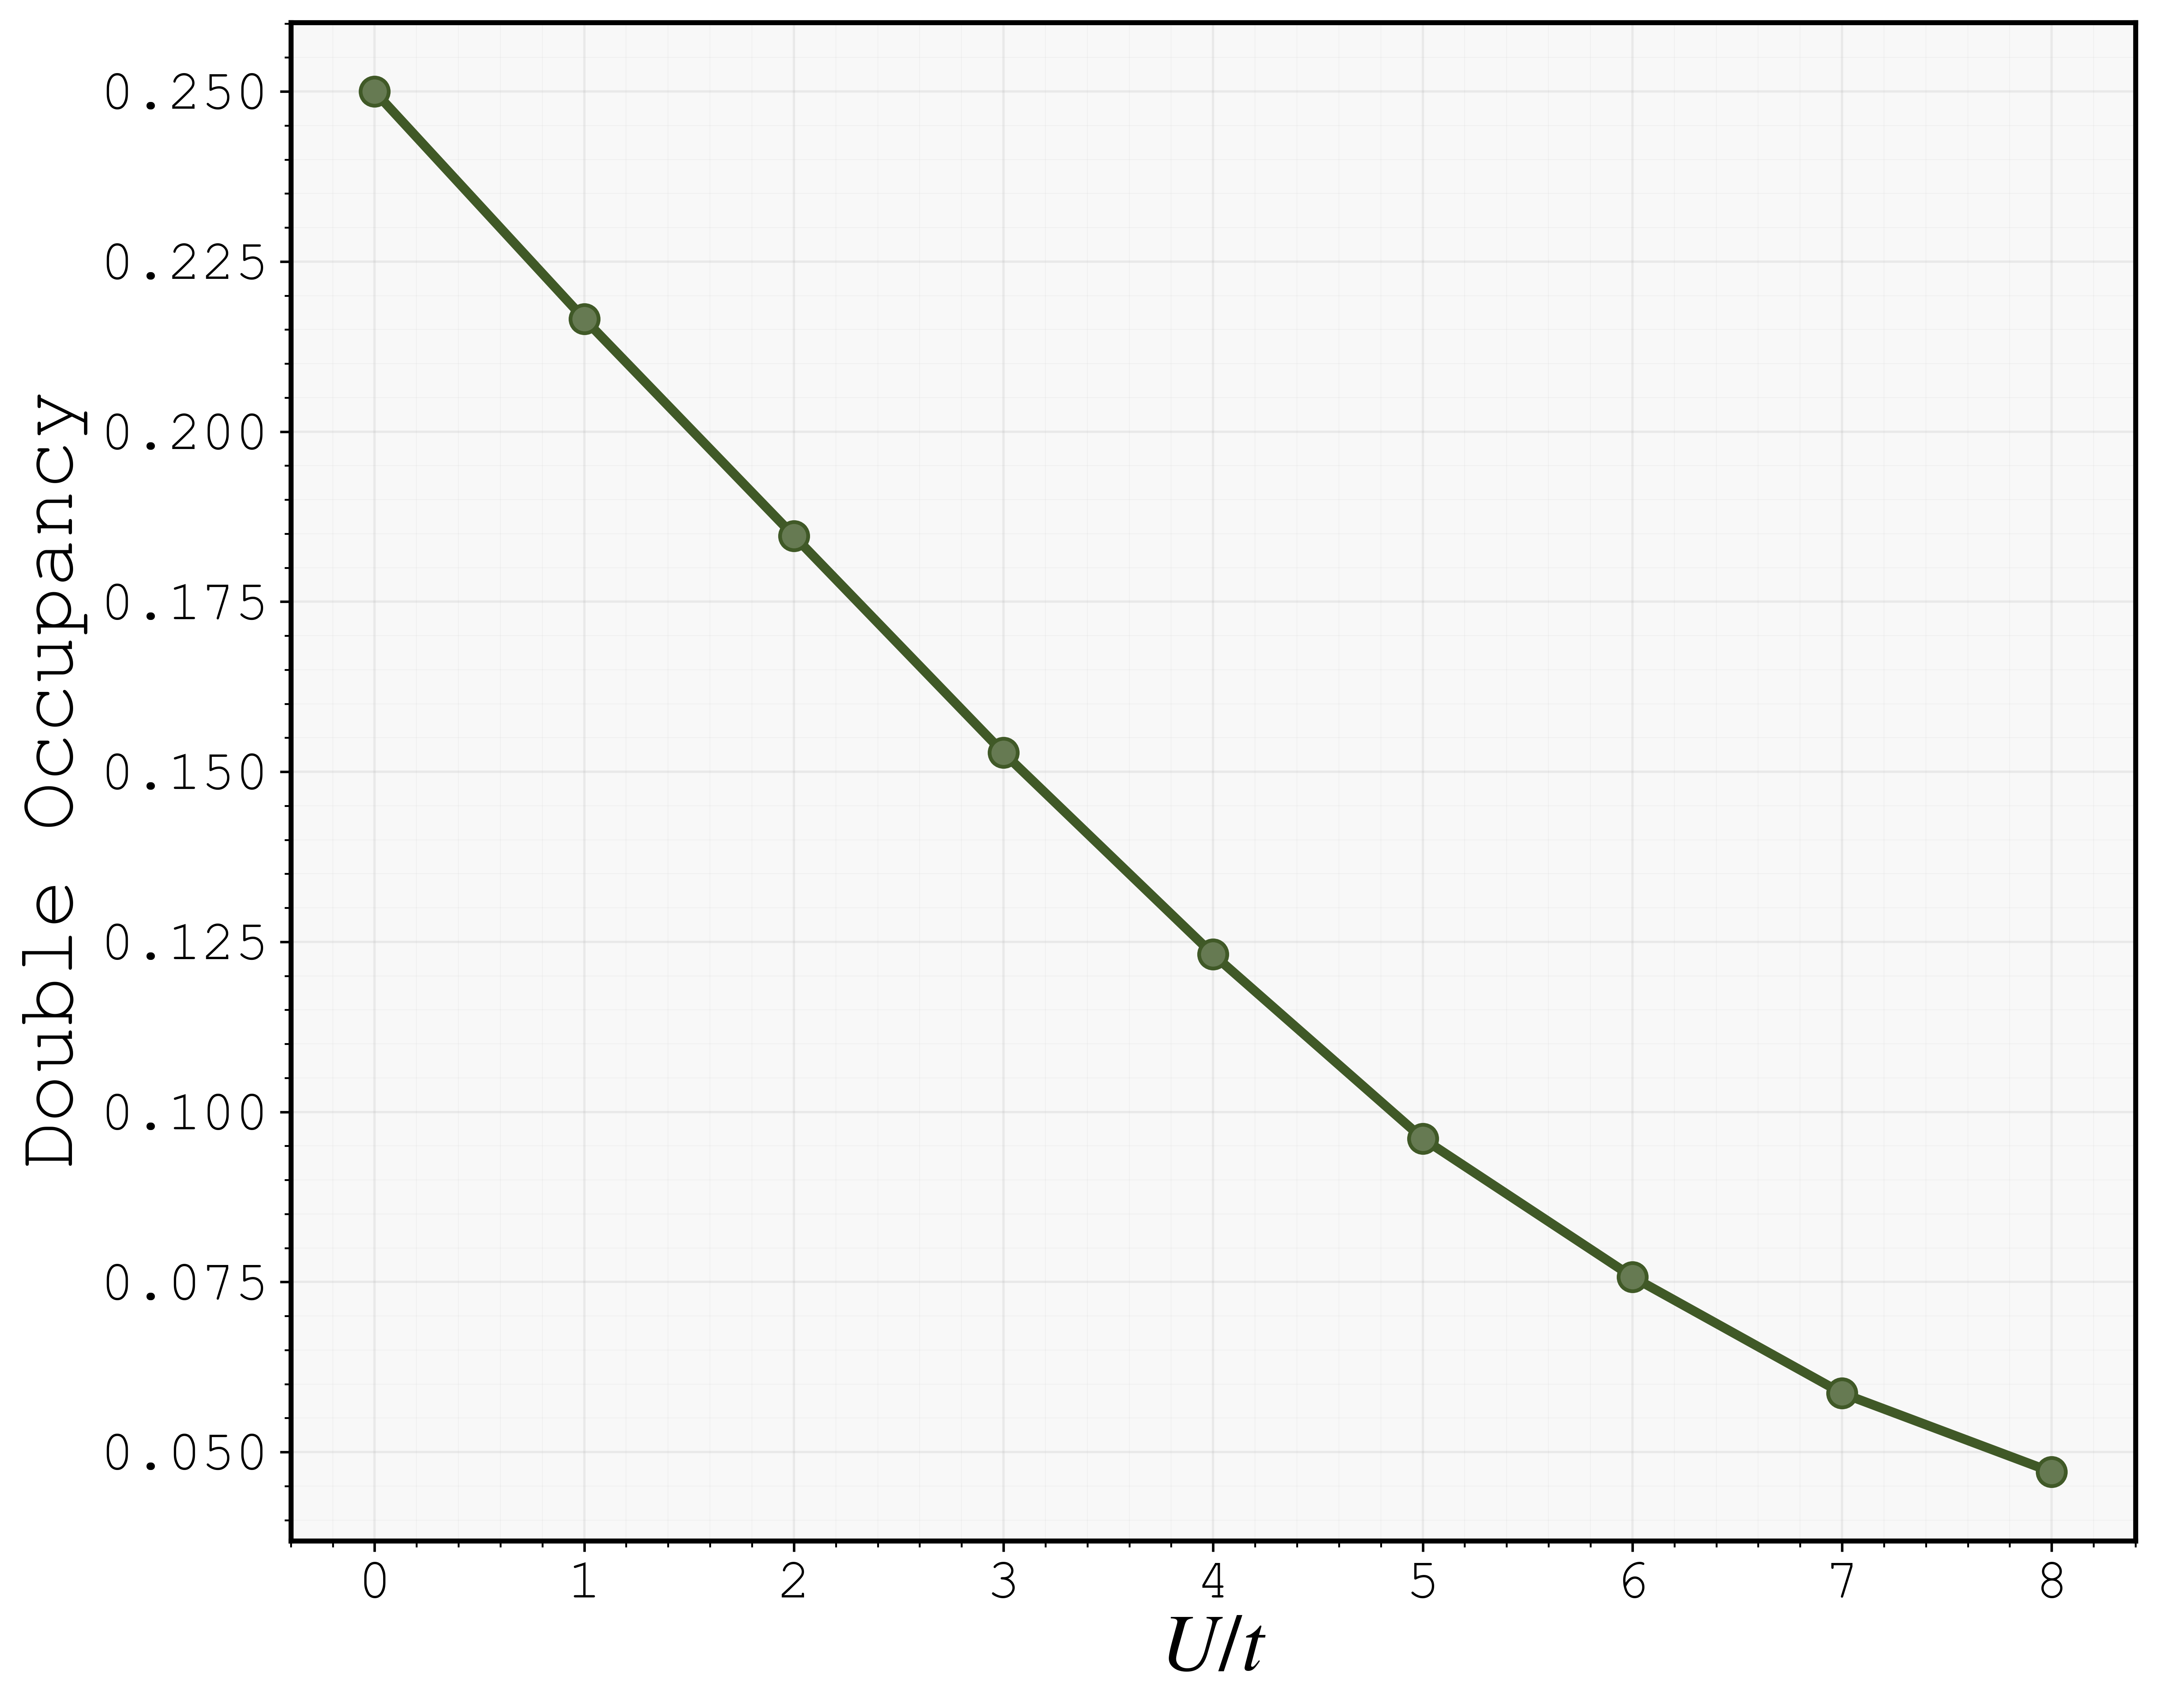
\includegraphics[width=0.32\textwidth]{uploads/double_occupancy_plot.png}
% \hfill
% 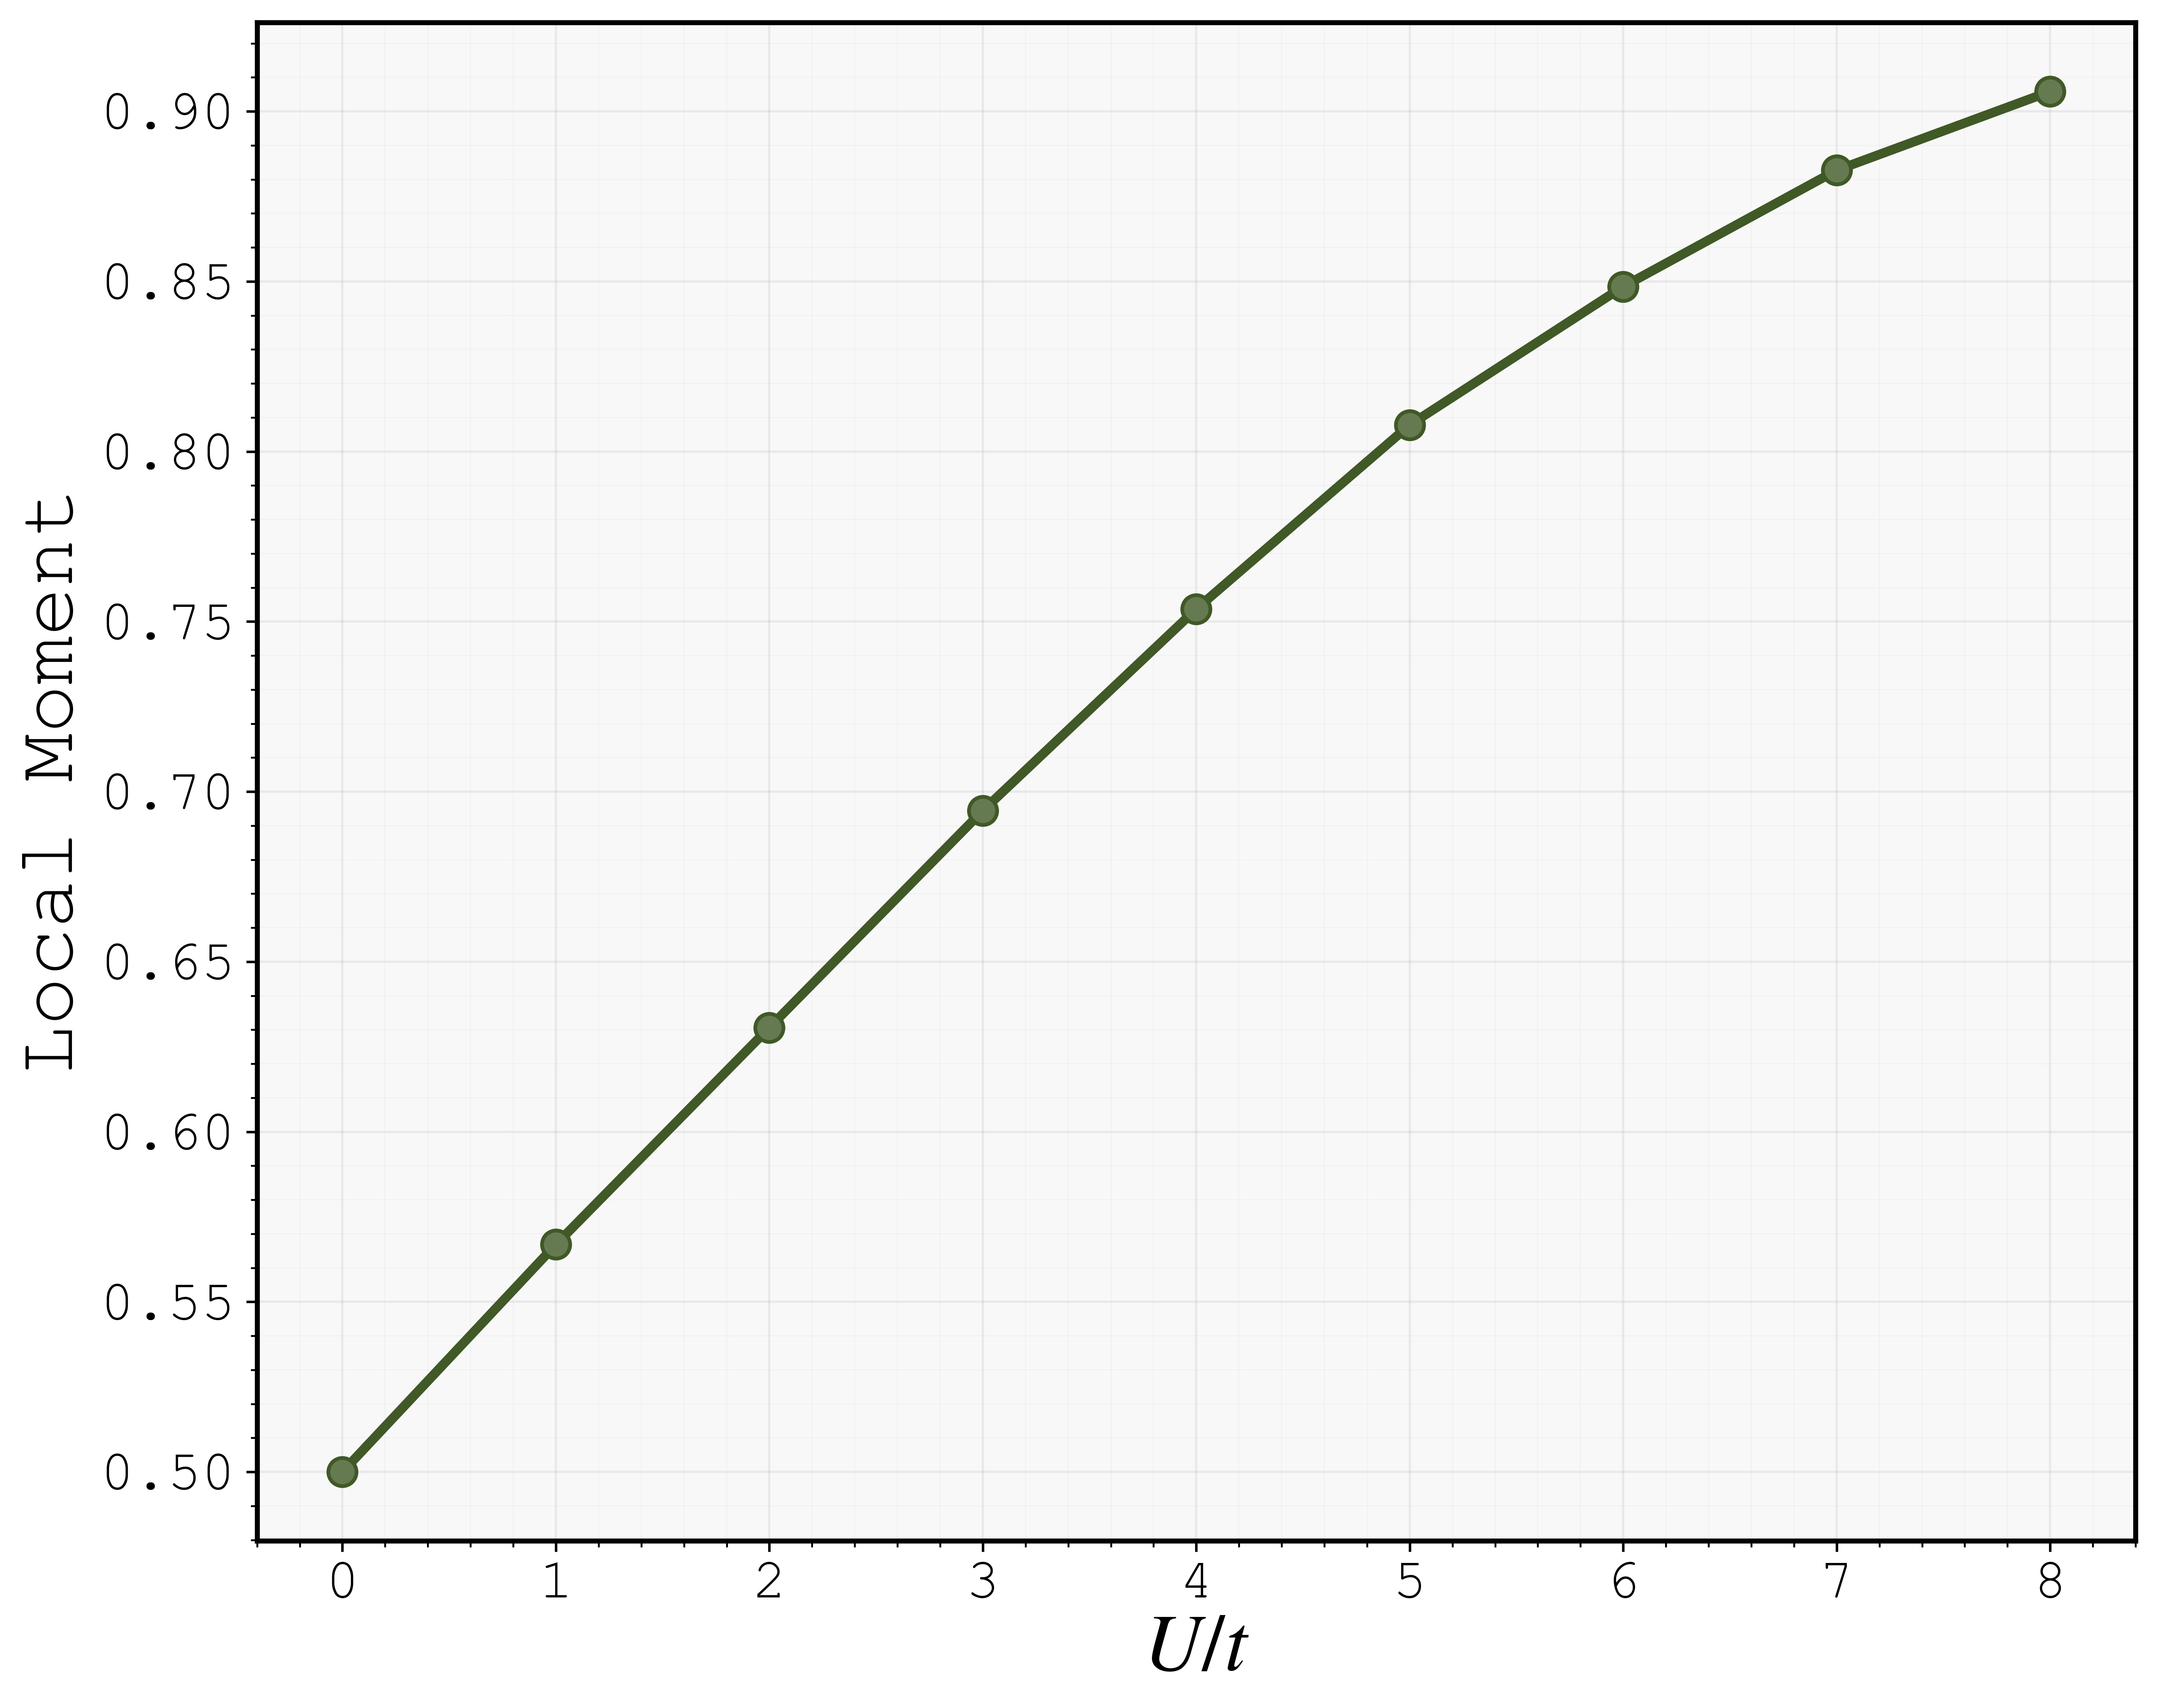
\includegraphics[width=0.32\textwidth]{uploads/local_moment_plot.png}
% \hfill
% \includegraphics[width=0.32\textwidth]{uploads/energy_plot.png}

% \caption{Results for the $4\times4$ Hubbard model at half filling and $\beta=4$. 
% (Left) Double occupancy decreases monotonically with increasing interaction strength, indicating suppression of charge fluctuations. 
% (Center) Local magnetic moment increases with $U/t$, reflecting the formation of localized spins. 
% (Right) Interaction energy exhibits a non-monotonic dependence due to the competition between interaction strength and double occupancy.}
% \label{fig:4x4_results}
% \end{figure*}

% As shown in Fig.~\ref{fig:4x4_results}, the double occupancy decreases monotonically with increasing interaction strength, while the local magnetic moment increases, indicating the formation of localized spins. The interaction energy exhibits a non-monotonic dependence on $U/t$, reflecting the competition between interaction strength and charge fluctuations.

% This behavior is a hallmark of the crossover from weakly correlated metallic behavior to a strongly correlated regime. In the strong-coupling limit, the system is better described in terms of localized moments, and the observed trends follow directly from the competition between hopping and on-site repulsion.

% The interaction energy rises initially with $U$ because each doubly occupied site becomes more expensive, but the rate of increase eventually slows as double occupancy is suppressed. This saturation-like behavior is physically reasonable and reflects the fact that the system cannot eliminate all charge fluctuations at finite temperature.

%----------------------------------------------------------
\section{Results and Physical Interpretation}
%----------------------------------------------------------

The results are consistent with the expected physics of the repulsive Hubbard model at half filling. Figure~\ref{fig:4x4_results} summarizes the $4\times4$ data set. As $U/t$ increases, double occupancy decreases because doubly occupied sites become energetically costly, while local moments grow because electrons preferentially avoid each other and occupy different sites.

\begin{figure*}[!t]
\centering

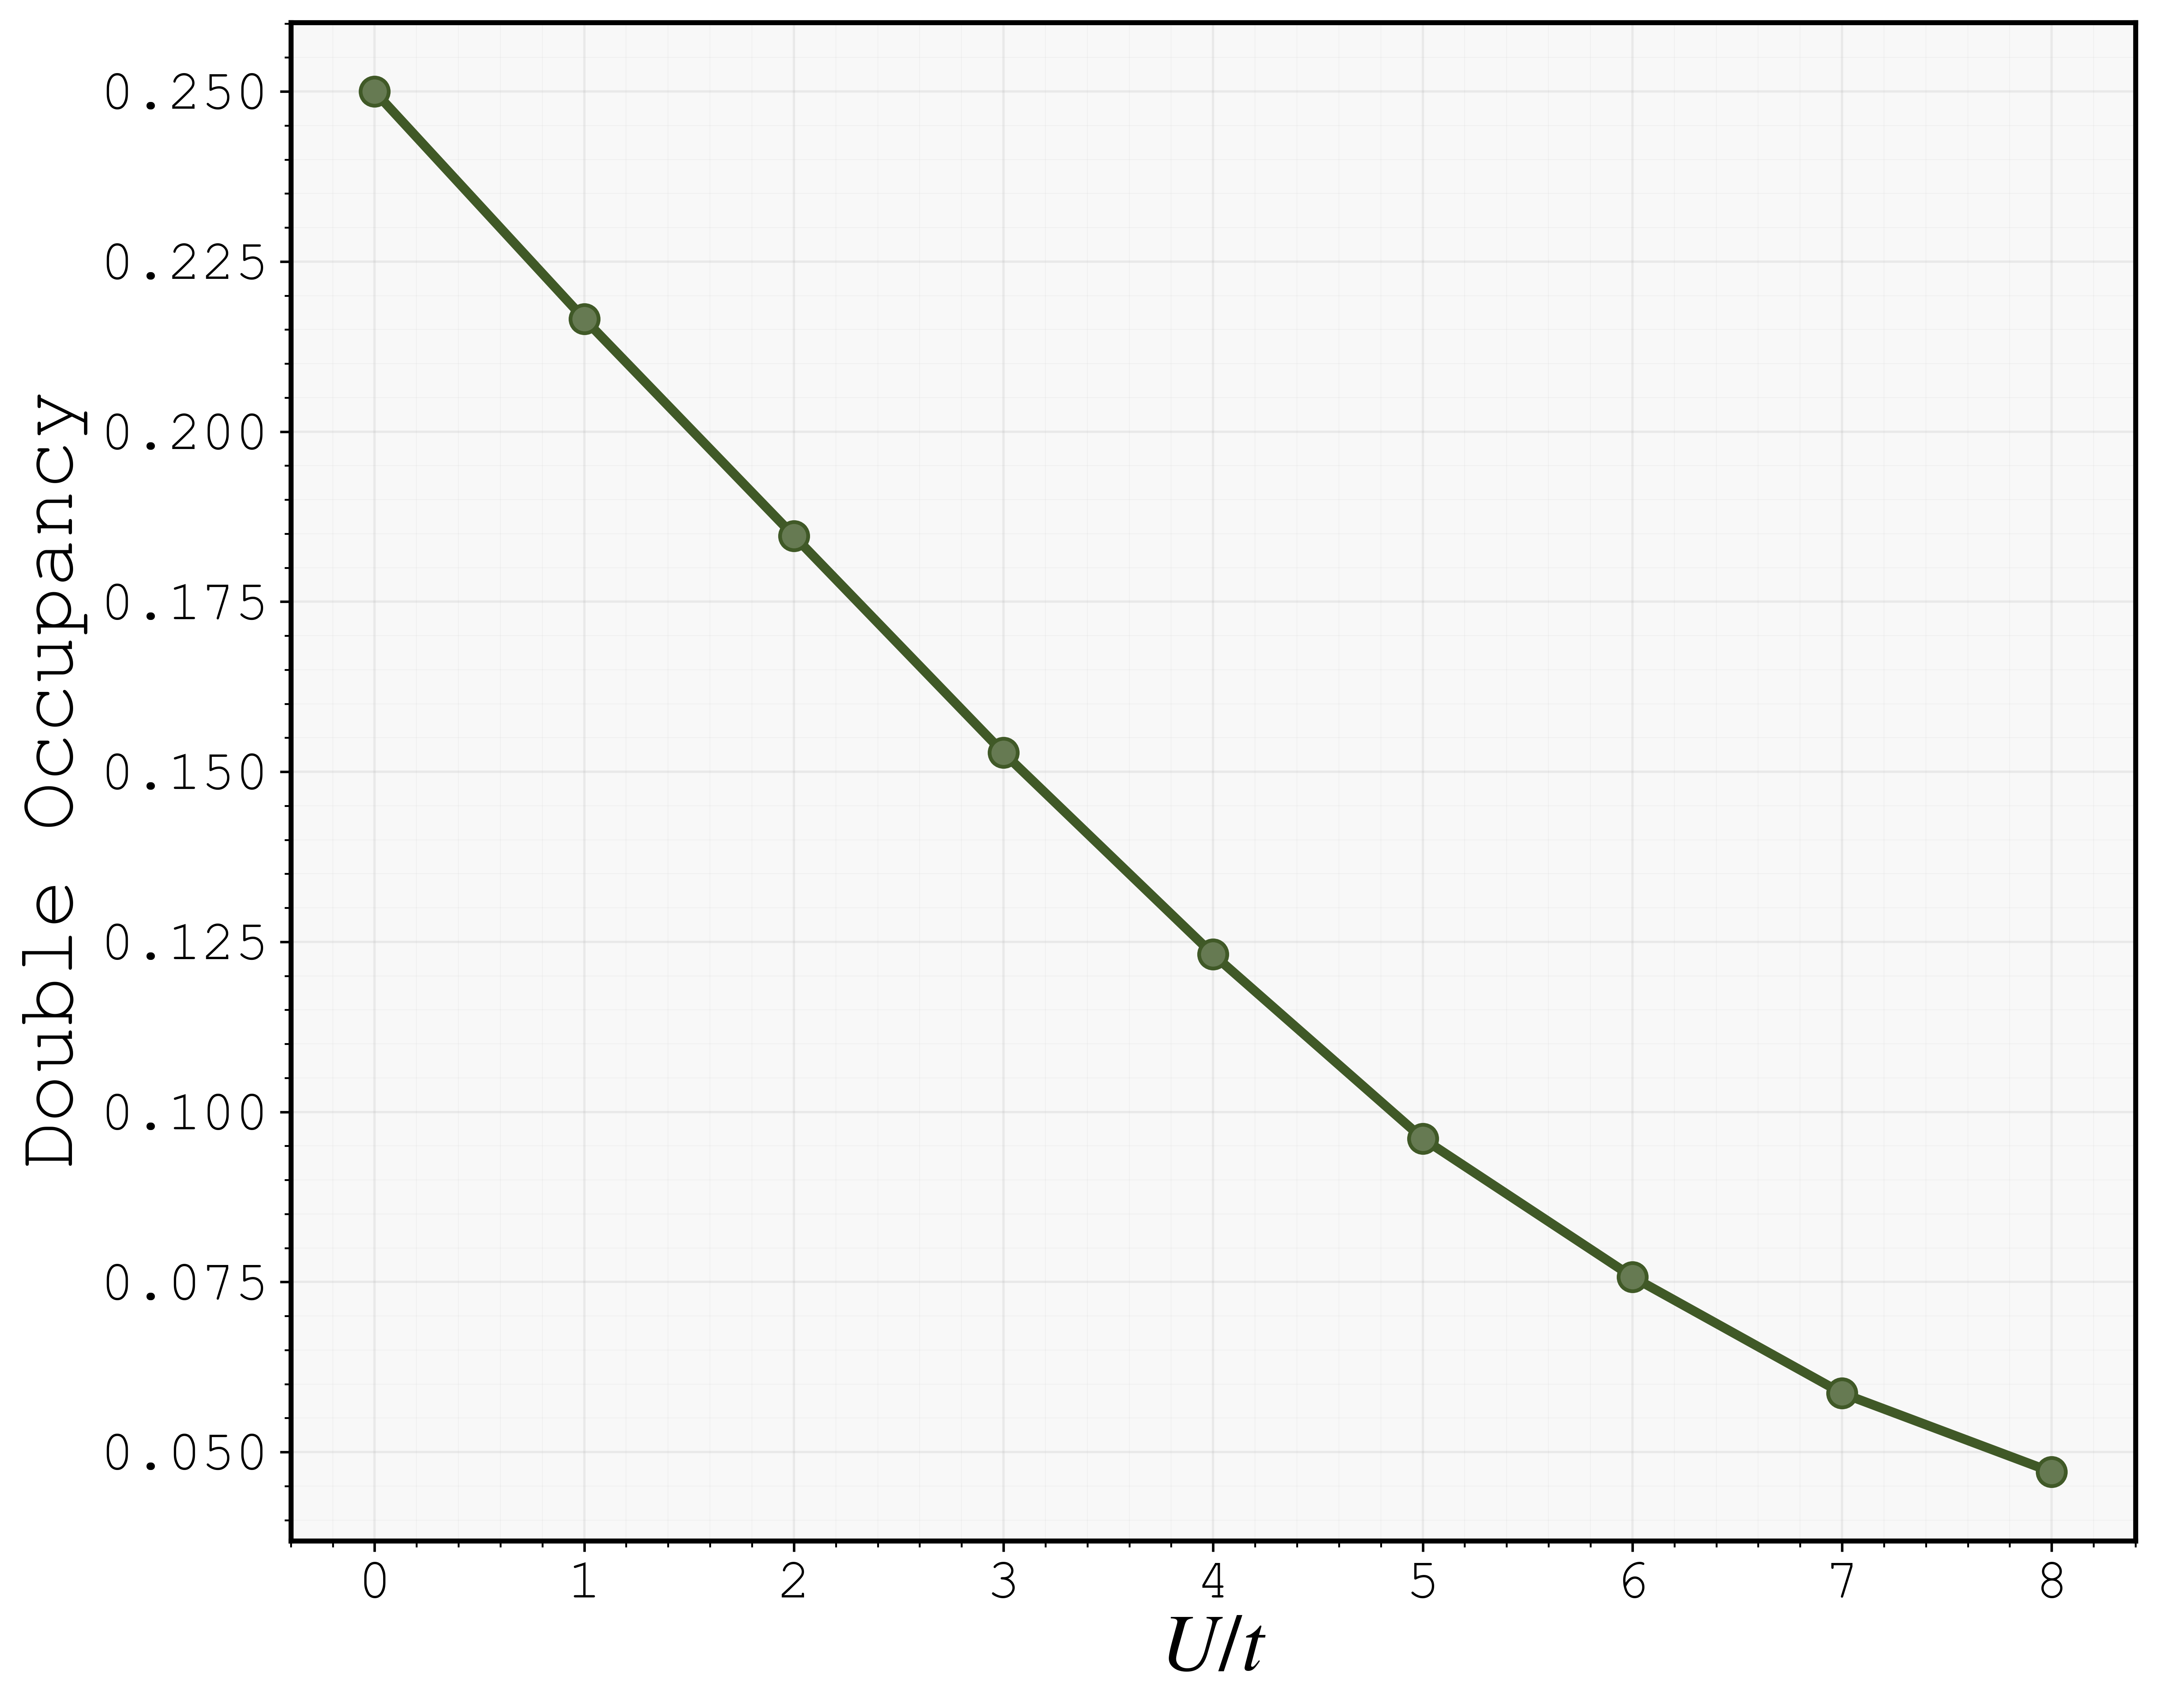
\includegraphics[width=0.32\textwidth]{uploads/double_occupancy_plot.png}
\hfill
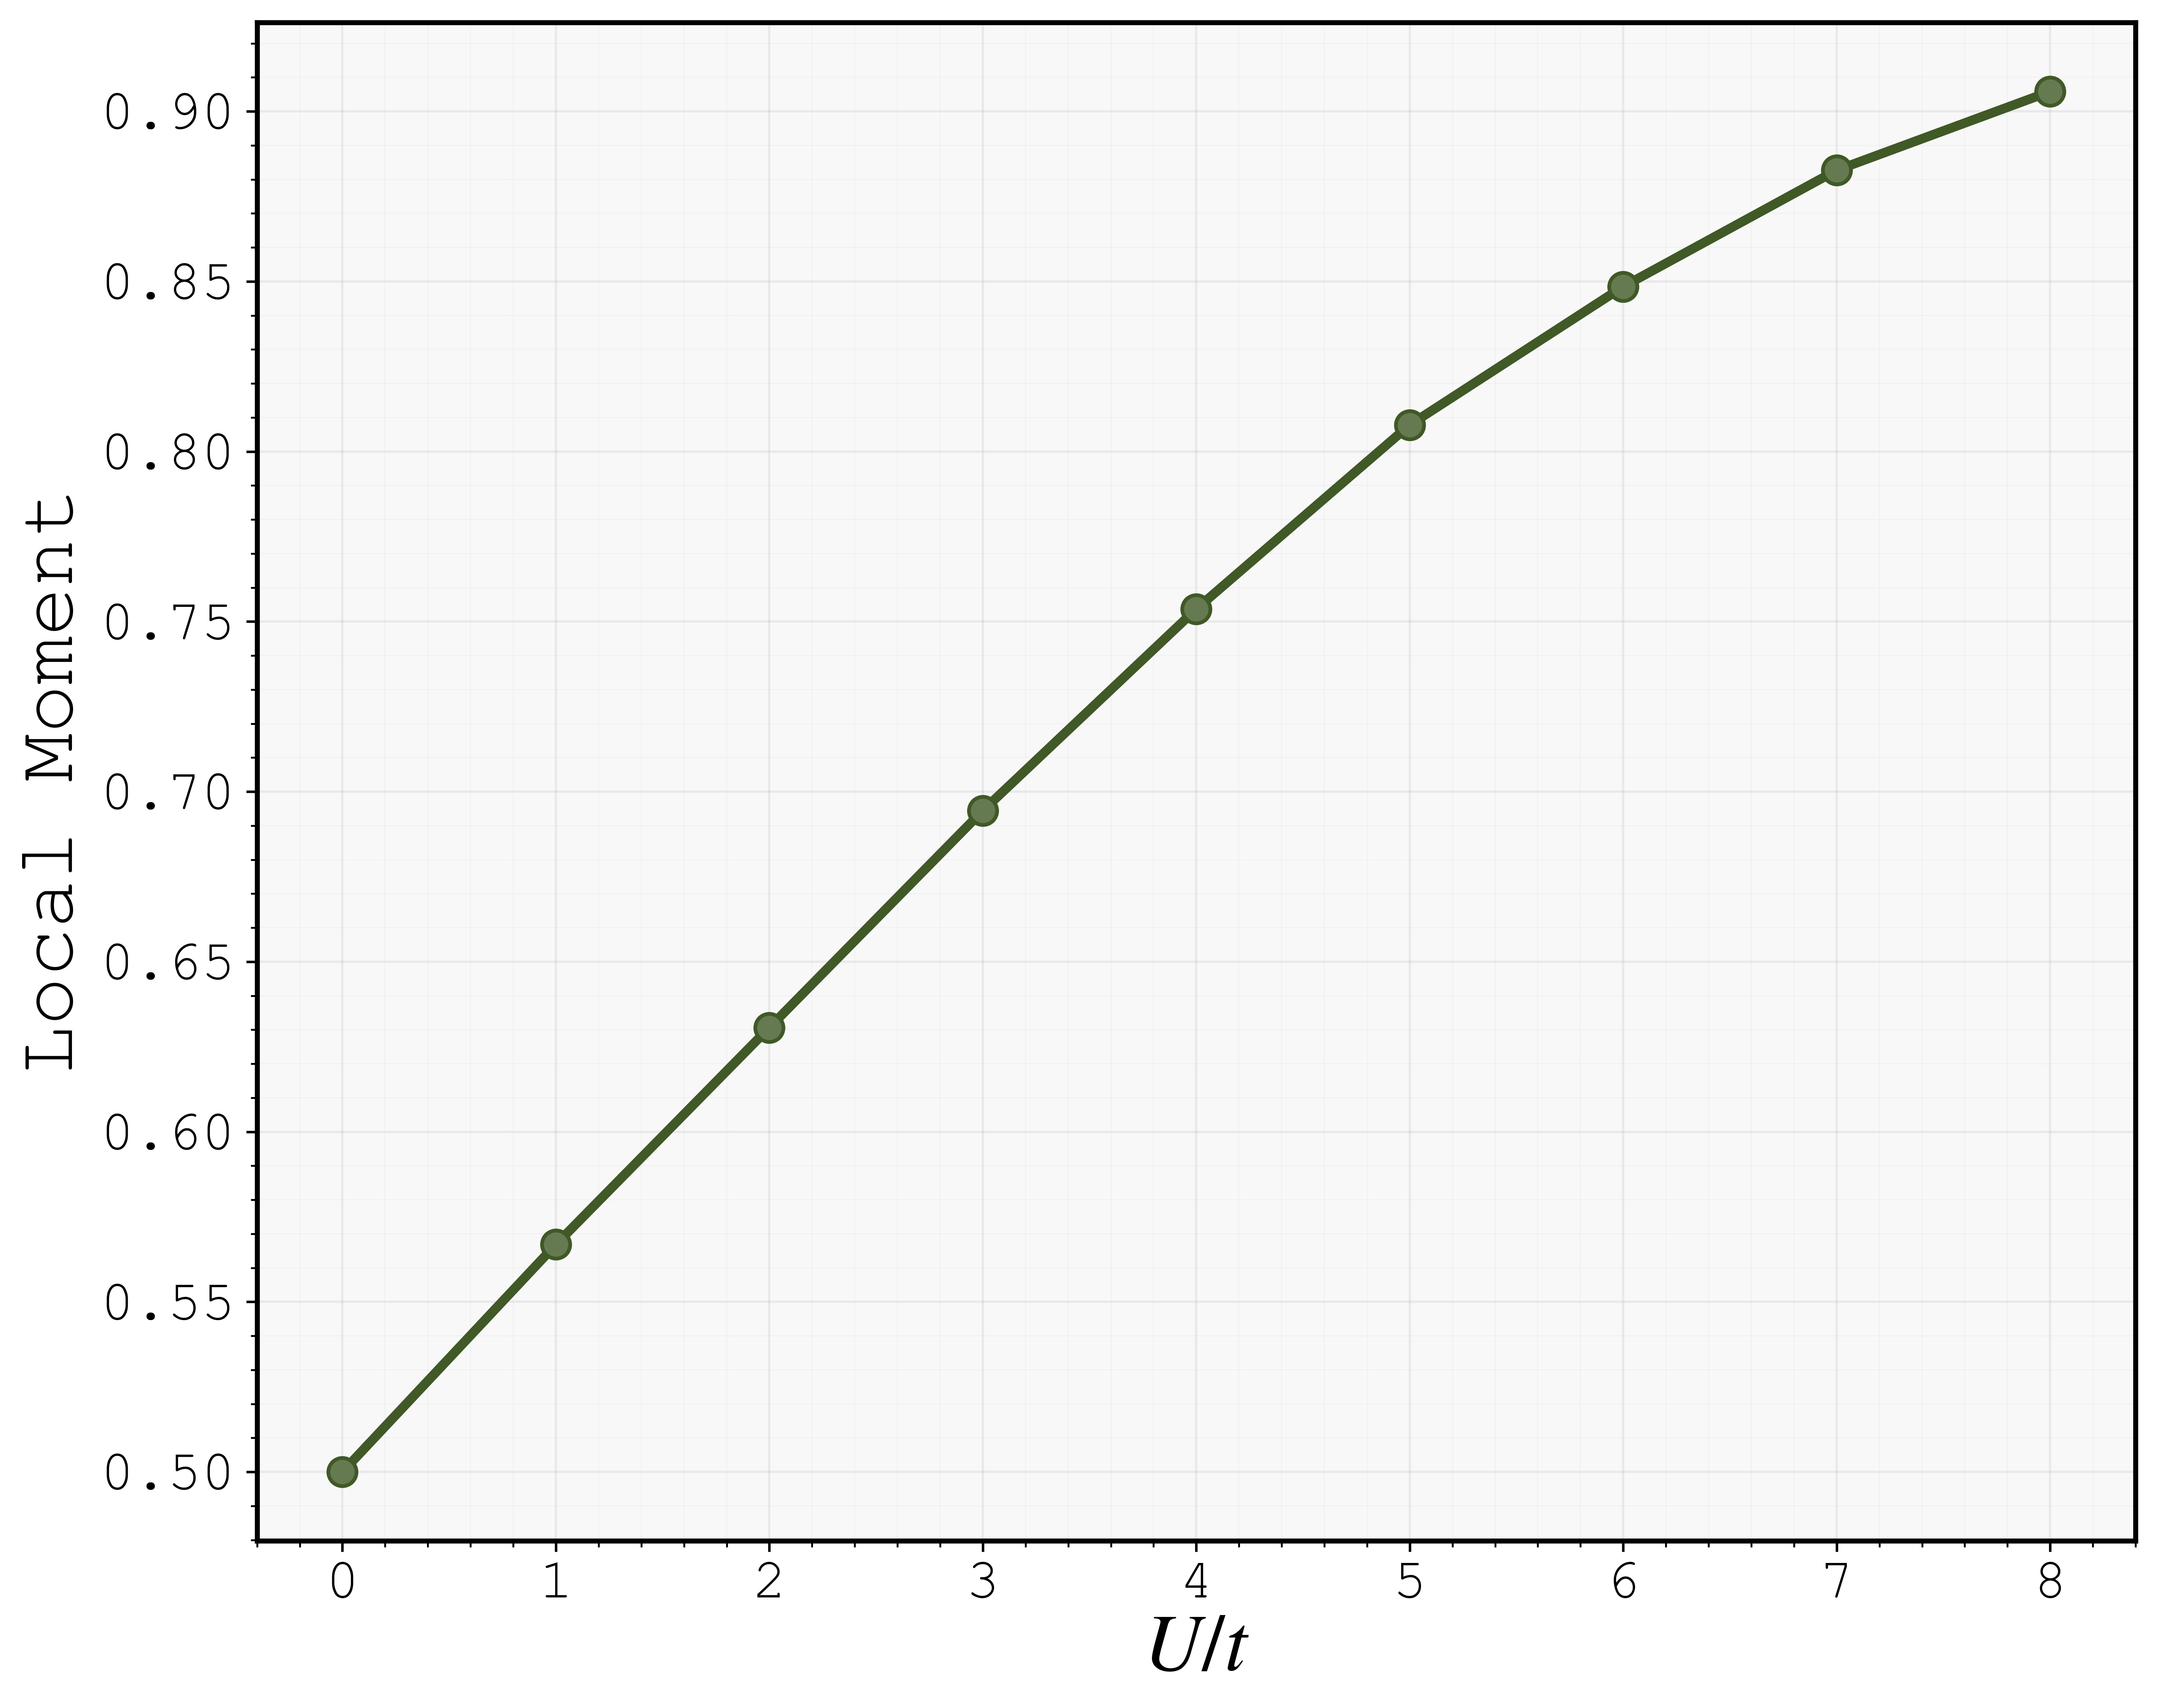
\includegraphics[width=0.32\textwidth]{uploads/local_moment_plot.png}
\hfill
\includegraphics[width=0.32\textwidth]{uploads/energy_plot.png}

\caption{Results for the $4\times4$ Hubbard model at half filling and $\beta=4$. 
(Left) Double occupancy decreases monotonically with increasing interaction strength, indicating suppression of charge fluctuations. 
(Center) Local magnetic moment increases with $U/t$, reflecting the formation of localized spins. 
(Right) Interaction energy exhibits a non-monotonic dependence due to the competition between interaction strength and double occupancy.}
\label{fig:4x4_results}
\end{figure*}

As shown in Fig.~\ref{fig:4x4_results}, the double occupancy decreases monotonically with increasing interaction strength, while the local magnetic moment increases, indicating the formation of localized spins. The interaction energy exhibits a non-monotonic dependence on $U/t$, reflecting the competition between interaction strength and charge fluctuations.

This behavior is a hallmark of the crossover from weakly correlated metallic behavior to a strongly correlated regime. In the strong-coupling limit, the system is better described in terms of localized moments, and the observed trends follow directly from the competition between hopping and on-site repulsion.

The interaction energy rises initially with $U$ because each doubly occupied site becomes more expensive, but the rate of increase eventually slows as double occupancy is suppressed. This saturation-like behavior is physically reasonable and reflects the fact that the system cannot eliminate all charge fluctuations at finite temperature.

%----------------------------------------------------------
\subsection{Finite-Size Effects: Double Occupancy}
%----------------------------------------------------------

To assess finite-size effects, we compare the double occupancy 
$D = \langle n_{\uparrow} n_{\downarrow} \rangle$ obtained from 
$2 \times 2$ and $4 \times 4$ lattice simulations, as shown in Fig.~\ref{fig:double_occ_comparison}.

\begin{figure}[!h]
    \centering
    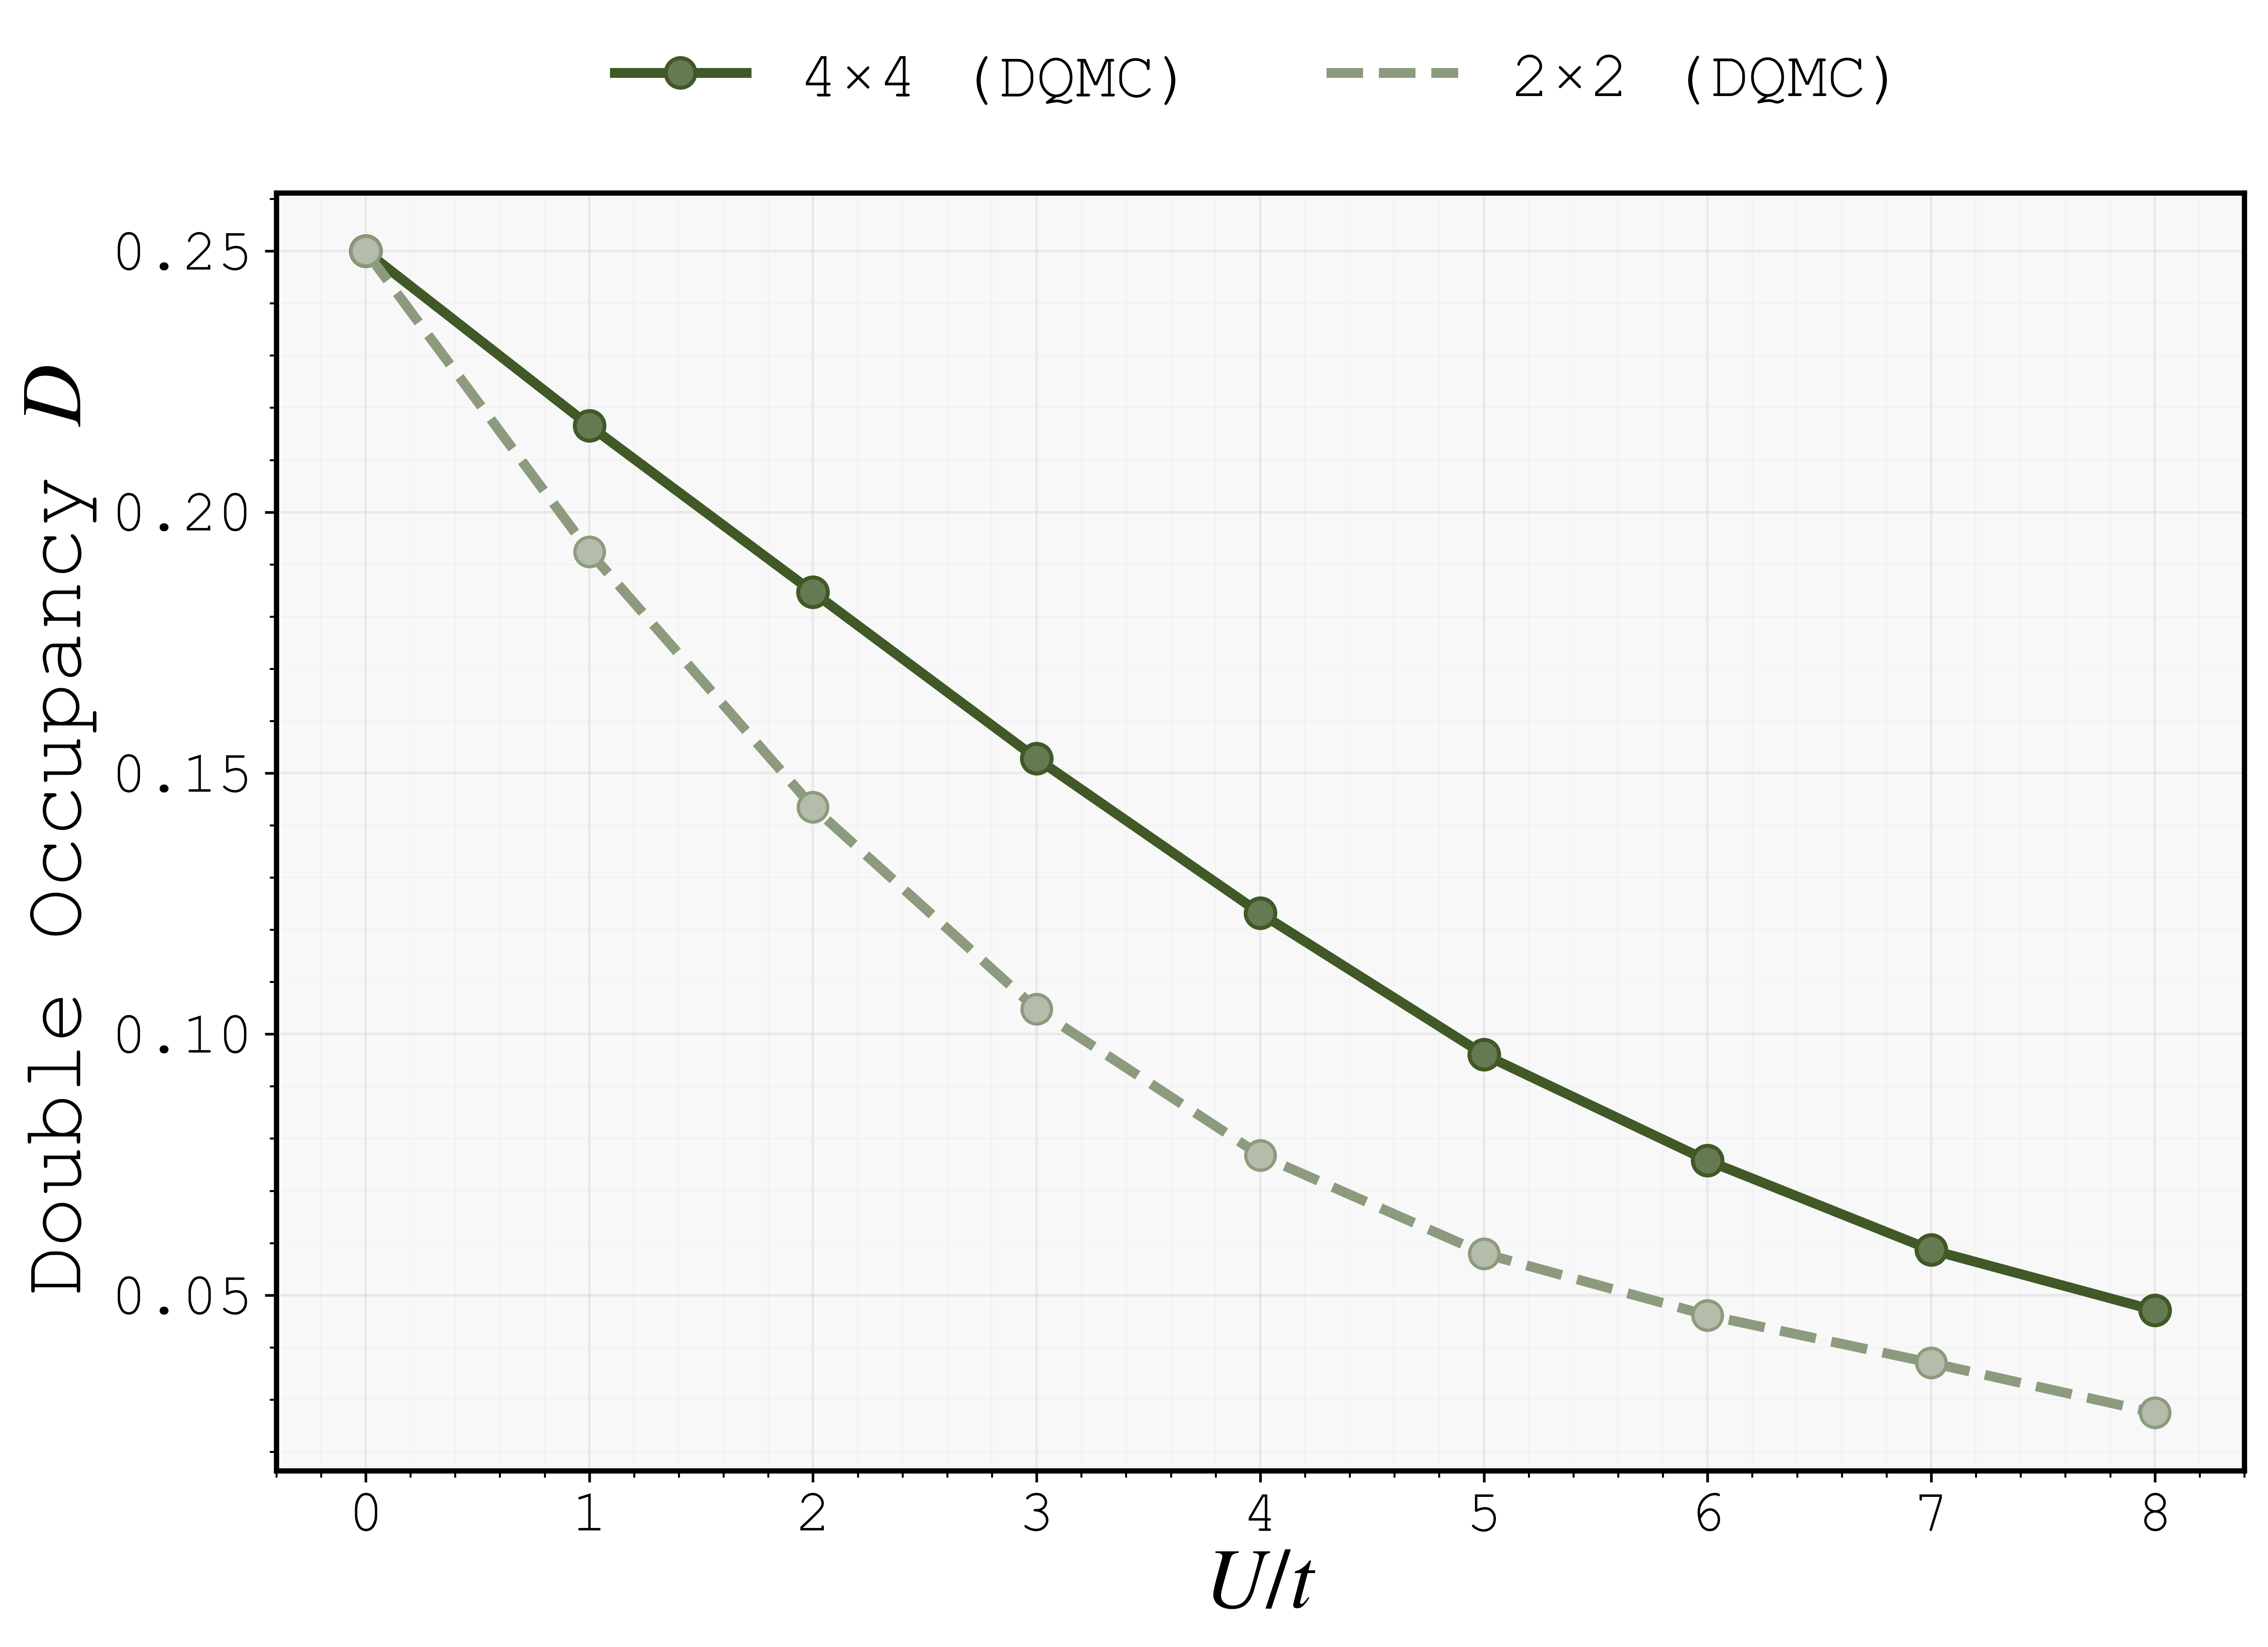
\includegraphics[width=0.9\columnwidth]{uploads/double_occupancy_2x2_vs_4x4.png}
    \caption{Comparison of double occupancy as a function of $U/t$ 
    for $2 \times 2$ and $4 \times 4$ lattices.}
    \label{fig:double_occ_comparison}
\end{figure}

As shown in Fig.~\ref{fig:double_occ_comparison}, the double occupancy 
decreases monotonically with increasing interaction strength for both 
system sizes. However, the $2 \times 2$ system consistently exhibits 
lower double occupancy than the $4 \times 4$ system, indicating stronger 
apparent correlation effects in smaller lattices.

The deviation between the two curves is most pronounced at intermediate 
values of $U/t$, where the competition between kinetic energy and 
interaction effects is strongest. This highlights the role of finite-size 
effects, as smaller systems lack sufficient spatial degrees of freedom 
to accurately capture fluctuations.

In the strong-coupling limit ($U/t \gg 1$), both curves approach similar 
values, suggesting convergence toward a regime dominated by local physics. 
Overall, these results indicate that while the $2 \times 2$ system captures 
qualitative trends, the $4 \times 4$ lattice provides a more reliable 
approximation to the thermodynamic limit.

%----------------------------------------------------------
\section{Trotter Error and Extrapolation}
%----------------------------------------------------------

Because the first-order Trotter decomposition introduces a systematic error of order $\Delta\tau$, observables should ideally be computed at several values of $\Delta\tau$ and extrapolated to the continuum limit. A standard linear extrapolation form is

\begin{equation}
O(\Delta\tau) = O_0 + A\,\Delta\tau,
\end{equation}

where $O_0$ is the extrapolated value at $\Delta\tau \to 0$. This procedure is particularly important when high accuracy is required. Suggested timestep values for such a study include

\[
0.10,\quad 0.05,\quad 0.025.
\]

By comparing results at multiple values of $\Delta\tau$, one can estimate the size of the systematic error and verify that the chosen timestep is sufficiently small. Note that if a symmetric (second-order) Trotter splitting were used instead, the leading error would be $O(\Delta\tau^2)$ and the extrapolation would be quadratic; the present asymmetric decomposition requires a linear fit.

%----------------------------------------------------------
\section{Finite-Size and Statistical Errors}
%----------------------------------------------------------

There are two major classes of uncertainty in DQMC calculations. The first is systematic error, which includes finite-size effects and Trotter discretization error. The second is statistical error, which comes from Monte Carlo sampling. On a $4\times4$ cluster, finite-size effects are especially important because the correlation length may be comparable to the system size.

Increasing the number of measurement sweeps reduces statistical fluctuations but does not remove finite-size bias. To improve reliability, one should simulate larger lattices such as $6\times6$ or $8\times8$ and perform size scaling. Similarly, one should verify convergence with respect to the equilibration time and the time-step discretization.

%----------------------------------------------------------
\section{Conclusion}
%----------------------------------------------------------

This project implements a DQMC simulation of the two-dimensional Hubbard model and reproduces the expected correlation-driven trends in a finite lattice calculation. The numerical results support the physical picture of suppressed double occupancy and enhanced local moments as the interaction strength increases. The report also clarifies the theoretical basis of the Hubbard model, the imaginary-time DQMC formulation, and the numerical stabilization needed for reliable simulation.

The implementation was validated against exact diagonalization results for a $2\times2$ lattice, providing confidence in the correctness of the algorithm. The current implementation already stores imaginary-time displaced Green's functions $G^\sigma(\tau, 0)$ for all time slices, which opens the door to future computation of dynamic spin and charge susceptibilities without algorithmic changes.

Future improvements should include full kinetic-energy measurements, larger lattices, systematic Trotter extrapolation, and improved statistics. These additions would make the study substantially more complete and would allow a more detailed comparison with known results for the half-filled two-dimensional Hubbard model \cite{Yao2018DQMC,white1989}.

%----------------------------------------------------------
\appendix
\section{Brief Derivations and Implementation Note}
%----------------------------------------------------------

This appendix collects two short derivations that are useful for DQMC but were not written out in the main text.

\subsection{Why the Suzuki--Trotter factorization works}

Let $H=K+V$, where $K$ is the hopping part and $V$ is the on-site interaction. For a small imaginary-time step $\Delta\tau$, the Baker--Campbell--Hausdorff formula gives

\begin{equation}
e^{-\Delta\tau K}e^{-\Delta\tau V}
=
\exp\!\bigg[-\Delta\tau(K+V)+\frac{(\Delta\tau)^2}{2}[K,V]+O\!\big((\Delta\tau)^3\big)\bigg].
\end{equation}
\\
Because $K$ and $V$ do not commute, the commutator term is nonzero. Repeating this product over $L=\beta/\Delta\tau$ slices gives

\begin{equation}
\left(e^{-\Delta\tau K}e^{-\Delta\tau V}\right)^L
=
e^{-\beta H}+O(\beta\,\Delta\tau),
\end{equation}

which explains why the asymmetric decomposition used here has a leading linear Trotter error. A symmetric splitting,

\begin{equation}
e^{-\Delta\tau K/2}e^{-\Delta\tau V}e^{-\Delta\tau K/2},
\end{equation}

would cancel the leading commutator contribution and reduce the global error to $O\big(\beta(\Delta\tau)^2\big)$.

\subsection{Checking the discrete Hubbard--Stratonovich identity}

At half filling it is convenient to rewrite the interaction on one site as

\begin{equation}
U n_{\uparrow}n_{\downarrow}
=
U\left(n_{\uparrow}n_{\downarrow}-\frac{n_{\uparrow}+n_{\downarrow}}{2}\right)
+\frac{U}{2}(n_{\uparrow}+n_{\downarrow}).
\end{equation}

The nontrivial part is then decoupled through an Ising field $s=\pm1$ by demanding

\begin{equation}
e^{-\Delta\tau U(n_\uparrow n_\downarrow-\frac{n_\uparrow+n_\downarrow}{2})}
=
\frac{1}{2}\sum_{s=\pm1}e^{\lambda s(n_\uparrow-n_\downarrow)}.
\end{equation}

This identity can be verified directly by evaluating the four local occupations $(n_\uparrow,n_\downarrow)=(0,0),(1,0),(0,1),(1,1)$. The left-hand side equals $1$, $e^{\Delta\tau U/2}$, $e^{\Delta\tau U/2}$, and $1$, respectively. The right-hand side equals $1$, $\cosh\lambda$, $\cosh\lambda$, and $1$. Matching the singly occupied states therefore requires

\begin{equation}
\cosh\lambda=e^{\Delta\tau U/2},
\end{equation}

which is the relation used in the simulation. The quartic interaction is thus replaced by a sum over binary auxiliary fields coupled linearly to the spin density $n_\uparrow-n_\downarrow$.

\subsection{Implementation note}

Parts of the final simulation code were adapted and modified from Dylan Jones's \texttt{dqmc} repository (MIT License), available at \href{https://github.com/dylanljones/dqmc}{github.com/dylanljones/dqmc}.

%----------------------------------------------------------
\section{References}
%----------------------------------------------------------

\printbibliography[heading=none]

\end{document}